\documentclass[10pt]{article}

% amsmath package, useful for mathematical formulas
\usepackage{amsmath}
% amssymb package, useful for mathematical symbols
\usepackage{amssymb}

% graphicx package, useful for including eps and pdf graphics
% include graphics with the command \includegraphics
\usepackage{graphicx}

% cite package, to clean up citations in the main text. Do not remove.
\usepackage{cite}

\usepackage{color} 

% Use doublespacing - comment out for single spacing
\usepackage{setspace} 
\doublespacing

% Text layout
\topmargin 0.0cm
\oddsidemargin 0.5cm
\evensidemargin 0.5cm
\textwidth 16cm 
\textheight 21cm

% Bold the 'Figure #' in the caption and separate it with a period
% Captions will be left justified
\usepackage[labelfont=bf,labelsep=period,justification=raggedright]{caption}

% Use the PLoS provided bibtex style
\bibliographystyle{plos2009}

% Remove brackets from numbering in List of References
\makeatletter
\renewcommand{\@biblabel}[1]{\quad#1.}
\makeatother


% Leave date blank
\date{}

\pagestyle{myheadings}
%% ** EDIT HERE **

\usepackage{multirow}

%% ** EDIT HERE **
%% PLEASE INCLUDE ALL MACROS BELOW

% figure files reside in the figures/ directory
\graphicspath{
{figures/}
}


\usepackage{color}
\usepackage[usenames,dvipsnames]{xcolor}
\usepackage{ulem}

\definecolor{dkred}{rgb}{0.75,0,0}
\definecolor{dkgreen}{rgb}{0,0.5,0}
\definecolor{dkblue}{rgb}{0,0,0.75}
\definecolor{dkpurple}{rgb}{.375,0,.375}
\definecolor{gray}{rgb}{0.5,0.5,0.5}

\newcommand{\removed}[1]{{\color{dkred}\sout{#1}}}
\newcommand{\drew}[1]{{\color{dkgreen}#1}}
\newcommand{\fred}[1]{{\color{dkblue}#1}}
\newcommand{\steph}[1]{{\color{dkpurple}#1}}

%% END MACROS SECTION

\begin{document}

% Title must be 150 characters or less
\begin{flushleft}
{\Large
\textbf{Spatially explicit model of the lymphocyte diaspora in influenza-infected lung reveals thresholds on chemokine directed migration (SUPPLEMENT)}
}
% Insert Author names, affiliations and corresponding author email.
\\
Drew Levin$^{1,\ast}$, 
Stephanie Forrest$^{1}$, 
Soumya Banerjee$^{1}$,
Candice Clay$^{2}$, 
Melanie Moses$^{1}$, 
Frederick Koster$^{1,2}$
\\
\bf{1} Department of Computer Science, University of New Mexico, Albuquerque, NM, USA
\\
\bf{2} Lovelace Respiratory Research Institute, Albuquerque, NM, USA
\\
$\ast$ E-mail: Corresponding drew@cs.unm.edu
\end{flushleft}


% You may title this section "Methods" or "Models". 
% "Models" is not a valid title for PLoS ONE authors. However, PLoS ONE
% authors may use "Analysis" 
\section{Models}

\subsection{Estimating chemokine production rates}

We estimate chemokine production rates, `r', by adapting the delay differential equation model of influenza infection described in \cite{Mitchell2011} \drew{Eq. 1} by adding one new equation ($\dot{C}=r I_{1 \tau_3}-dC$) to model chemokine production.  Initial population sizes and parameter values are taken from the previous study.
{\footnotesize
\begin{equation}
\begin{aligned}
\dot{T} &= - \beta T V \\
\dot{I_1} &= \beta T V - \beta T_{\tau_1}V_{\tau_1} \\
\dot{I_2} &= \beta T_{\tau_1}V_{\tau_1} - \delta I_2 \\
\dot{V} &= \frac{p}{1+eF} I_2  - \beta T V  \\
\dot{F} &=  I_{1 \tau_2} \\
\dot{C} &= r I_{1 \tau_3} - d C \\
\end{aligned}
\label{eq:dde}
\end{equation}
\vspace{.05in}
}

$\tau$ subscript variables denote delay terms, signifying the value is the population quantity in existence at time $t - \tau$.  Table 1 summarizes population and parameter values and descriptions.  Strain-specific values for $r$ were found by fitting the equations to experimental data (see Results and Table 3).


\subsection{T cell production rate}

We calculate the rate of production ($\sigma$) of CD8 T cells using a differential equation model from \cite{Miao2010}.  The equations model T cell production and subsequent search over an area of infected lung tissue.

{\footnotesize
\begin{equation*}
\label{EqS1}
\begin{aligned}
\dot{N_{c}} &= \sigma - \frac{r'^{2} \cdot N_{c}}{R^{2} \cdot t_{rc}} & \pi r'^{2} &= a \sqrt{I} + b \\
\dot{N'_{f}} &= \frac{(r'^{2} - r^{2}) \cdot N_{c}}{R^{2} \cdot t_{rc}} - \frac{v_{tcell}}{(r' - r) / 2} \hspace*{2cm}  & \pi r^{2} &= \pi r_{cell}^{2} \cdot I \\
\dot{N_{f}} &= \frac{r^{2} \cdot N_{c}}{R^{2} \cdot t_{rc}} + \frac{v_{tcell}}{(r' - r) / 2} \\
\dot{T} &= \rho T -\beta TV \\
\dot{I} &= \beta TV - \delta I - k_{e} N_{f} I \\
\dot{V} &= pI - \beta TV - \gamma (t) V \\
\gamma (t) &= \left\{ \begin{array}{rcl}
	1/\mbox{day} & \mbox{,}  & t < 5  \\
	3/\mbox{day} & \mbox{,} & t \geq 5  
	\end{array}\right. \\
\end{aligned}
\tag{S1}
\end{equation*}
}
\vspace{.05in}

$N_{c}$ is the number of circulating activated antigen-specific CD8 T cells, $N'_{f}$ is the number of circulating T cells that have found and exit into a region of lung tissue expressing chemokines, $N_{f}$ is the number of circulating T cells that have found an infected region. $T$ is the number of uninfected \textit{target} cells, $I$ is the number of productively infected cells, and $V$ is the viral titer in serum. The infected region is assumed to be of radius $r$ and is within a region expressing chemokines of radius $r'$ ($r  < r'$). The lung is modeled as a circular region with radius $R$. The area of the infected region is equal to the area of an infected cell (of radius $r_{cell}$) multiplied by the number of infected cells. See Fig. 1 for more details about the model.  The area of the region expressing chemokine was found to be related non-linearly to the number of infected cells ($\pi r'^{2} = a \sqrt{I} + b$) where $a$ and $b$ are constants that depend on the viral strain.  $a$ and $b$ were fit using 12 experimental runs of a spatial model implemented in CyCells.

Circulating CD8 T cells ($N_{c}$) are assumed to be released from lymph nodes at a constant rate $\sigma$ and circulate to the $N'_{f}$ population over a time defined by $t_{rc}$. We assume these circulating cells transition into $N'_{f}$ and $N_{f}$ at rates proportional to the areas of the chemokine expressing and infected regions relative to the whole lung area. 

The average time an exiting CD8 T cell takes to migrate to the infected region is equal to the difference in the radii between the two regions ($r' - r$) times the T cell speed, $v_{tcell}$.  Circulating cells that are in the chemokine expressing region ($N'_{f}$) move into the infected region after performing chemotaxis for that time. Target cells ($T$) become infected by virus at rate $\beta TV$, where $\beta$ is the rate constant characterizing infection. Infected cells ($I$) die at rate $\delta$ in addition to being lysed by T cells ($N_{f}$) at a rate $k_{e}$. Finally the viral titers ($V$) increase due to production of virus at rate $p$ by infected cells. Virus is also cleared due to uptake by infected cells (at a rate $- \beta TV$) and due to antibody (at a rate $\gamma (t)$ that changes after 5 days post infection). The initial viral titer was initialized to 10,000 PFUs and the initial number of target cells was one million. The initial number of infected cells is assumed to be zero. Parameter values are listed in Table S1 in Text S1.  This ODE was fit to data taken from \cite{Miao2010} using Matlab's \texttt{nlinfit} function in order to obtain a value for $\sigma$.  The final value was found to be 1,257 per hour.


\subsection{CyCells implementation details}

The CyCells modeling environment splits its populations into two types: cells and molecules.  Cells are considered to be unique agents and are modeled individually.  Conversely, molecules are represented as compartmentalized concentrations.  These compartments are arranged as a grid that covers the environment.  Each square in the grid contains a unique concentration of the given molecule.  Each type of  molecule is represented in a unique grid.

Molecular behavior is limited to diffusion and decay.  At each time step, CyCells decreases the concentration of each square in the grid according to the decay rate specified for the given molecule.  CyCells then diffuses the molecules by applying a discrete diffusion equation to each grid square, taking into account the specified diffusion constant and the concentrations in neighboring squares.

New molecules can be secreted by cell objects, such as an infected cell secreting new virus.  In this scenario CyCells calculates the amount of virus secreted per time step, based upon the cell's defined production rate, and then adds this quantity to the grid square that overlaps the secreting cell.  If a cell ingests a molecule, it will subtract the appropriate concentration from the grid square it overlaps.  If the concentration at that square is not enough to represent a full molecule, concentration will be removed from neighboring squares in an ever expanding diamond until the total concentration is equal to a single molecule.

Cells will measure the local concentration at their position by calculating a linearly interpolated combination of the concentrations in the grid squares surrounding the cell in instances where cell behavior depends on the local molecular concentration.


\subsection{Model implementation details}

An overview of the model implementation is shown in Fig. 2.  The model is initialized with one virus-secreting cell placed in the middle of a 2-dimensional sheet of hexagonally-tiled epithelial cells (288,212 total cells).  The sheet measures 5$mm$ per side, which is large enough to contain the infection (Fig. 5).  The molecular grid (Text S1 1.3) is initialized with a resolution of 20$\mu m$.  Each time step of the model represents 6 seconds.

Healthy cells transition to virus-incubating based on a probability that scales linearly with the local virus concentration.   When a cell `becomes infected' it removes the amount of viral concentration equal to a single virion. 

Virus-incubating cells idle for 10 hours (with standard deviation $\sigma=1$ hour) and then transition to virus-secreting cells.  Virus-incubating cells also begin to secrete chemokine after 8 hours (except for aH5N1 which only secretes RANTES after a 16 hour delay).  

Virus-secreting cells secrete both virus and chemokine (the RANTES portion of the chemokine production is added in 16 hours after the initial infection) and die after 1,000 minutes of production (16.7 hours).  Virus-secreting cells will also probabilistically transition to apoptizing cells in the presence of T cells (defined by the existence of a T cell within 2$\mu m$).  The number of T cells in the vicinity of the virus-secreting cell has no effect on the rate that apoptosis is induced in the model.

Apoptizing cells secrete virus and chemokine for one hour and then die.

T cells are added to the model at a constant rate of 1,257 per hour (Text S1 1.1).  Because the model environment is only a small portion of the entire lung (0.25\%), most of the T cells miss the model window and are not visually represented.  The T cells that miss recirculate and enter the lung at a new random location after a delay of six seconds.

The cells that enter the model window are placed at a random position and immediately check the local chemokine concentration.  If the concentration is above the sensitivity threshold, the T cells immediately transition to the chemotaxing state.  If not, the T cells recirculate and reenter the lung in a new location after a six second delay.  Recirculating T cells have a probabilistic decay rate that corresponds to a 3 day lifespan.  Recirculating T cells are not visually represented.  

Chemotaxing T cells move directly up the chemokine gradient until they find a local concentration maximum.  T cells probabilistically decay at a rate corresponding to a 2 hour lifespan.  Chemotaxing T cells have no effect other than inducing apoptosis in virus-secreting cells by proximity.


\subsection{Modeling Decisions}

\subsubsection{Two dimensional lung}

We model the lung as a two-dimensional system for several reasons.  Unlike the lymph node where dendritic cells and T cells navigate a three-dimensional volume, lung infection dynamics are confined to a thin tissue between capillary endothelial cells and alveolar epithelial cells.  Although these alveoli are segregated by the lung's acinar structure on a small scale, we do not represent this in the model because the spreading of influenza eventually ignores the boundaries between acinii.  Therefore our model does not incorporate this small-scale level of segregation.

\subsubsection{Uniform blood flow}

Our model assumes that blood flows uniformly through the lung vascular network.  It is possible that blood flow is increased in the direction of an infected region of the lung by local inflammation.  Thus our model may underestimate the recruitment efficiency of local inflammation and hyperemia.  If this is indeed the case, our model underestimates the effect of the immune response.

%\subsubsection{T cell velocity}
%\fred{T cell velocity in the lung is extremely difficult to measure.} \removed{Little is known of T cell chemotaxis speed in the lung.}  We give chemotaxing T cells a velocity of $3\mu m/s$ and T cells that are performing a random walk a velocity of $30\mu m/s$.  \removed{These values are faster that speeds found in other organs, such as the lymph node.  This is reasonable because T cells in the lung travel on top of a packed surface without needing to navigate through blood flow.  Furthermore, T cell speed has little effect on the model behavior as detailed below (S2.3).}  \fred{These rapid values estimate velocity of capillary blood flow in the extensive network of capillaries beyond the 14th bifurcation of the lung arterial system.  T cell velocity would be expected to be slower within interstitial tissue, but this was not modeled in most simulations.  In runs where velocity was varied over 5 orders of magnitude, including slow velocities measured in lymph node and skin by other authors, T cell velocity had little effect on model behavior and infection control as shown below (S2.3).}
%

%See Table~\ref{table:assumptions}.


% Results and Discussion can be combined.
\section{Results}

\subsection*{T cell sensitivity to chemokine}

The model simulates a chemokine gradient surrounding the infected focus (Fig. 5), based on the calculated per-infected cell secretion rate (Table 3) and known chemical parameters for a 10 kDa protein (Table 2).  T cell sensitivity depends on receptor density \cite{Desmetz2006} and this was assumed to be constant.

Because this parameter is unknown, we simulated T cell sensitivity levels ranging over 10 orders of magnitude.  Concentration-dependent behavior of cells responding to chemokine was the same over a wide range of concentrations from 0.01 pg/mL to 100 ng/mL (model variance is discussed in Text S1 2.1.).  Decreased recruitment was predicted only by supra-natural concentration sensitivity levels at and above 1 $\mu$g/mL.  We then set the sensitivity to 100 $ng/mL$ for all future runs (10 $nM$ concentration assuming a chemokine molecular weight of 10 $kDa$) \cite{Gao2003}.  

% Because more than one T cell at each infected epithelial cell would not increasing effective target cell death, there may be a threshold of immigrant T cells above which no additional control of viral replication is possible.


\subsection{Chemokine combinations}

Because aH5N1 has been shown to suppress the production of interferon \cite{Mitchell2011}, we hypothesize that it renders IP-10 ineffectual.  We hypothesize that this leads to the elevated RANTES secretion rates measured in aH5N1 compared to the other two strains (Table 3).  Because of this behavior IP-10 was not included in the aH5N1 model runs. 

T cell sensitivity depends on receptor density \cite{Desmetz2006} and this was assumed to be constant.  Thus, the chemokines in combination work additively in our model. 

Four models runs (both, IP-10, RANTES, and none) were performed for sH1N1 and pH1N1 strains and two runs (RANTES and none) for  aH5N1.  The runs show how the presence and/or absence of specific chemokines affect the simulated immune response (Fig.~S\ref{fig:chemokine}).  The lack of both chemokines leads to runaway infections in all three strains.  The presence of only RANTES is enough to contain the aH5N1 infection, but is weaker than IP-10 in both H1N1 strains.  In sH1N1 and pH1N1 simulations, IP-10 alone proves to be as effective as the combination of IP-10 and RANTES.  This suggests that RANTES does not play a significant role in infections that stimulate an IP-10 response due to the higher production rates of IP-10.  

%\drew{
%\subsection{T cell speed}
%
%\removed{T cell speed over bronchial epithelial cells is unknown.}\fred{T cell velocity within the capillary network and after diapedesis with the lung interstitial tissue is unknown.}  We tested values for T cell speed to measure the effect it had on the general infection dynamics (Fig.~S\ref{fig:speed}).  The results show that the difference in T cell speeds is small, although there does appear to be an discernible effect on the infection during \removed{the early phase of the T cell response} \fred{the initial appearance of activated T cell migration between days 5 and 7 post infection.}.
%}

% The bibtex filename
\bibliography{references}

\pagebreak

\section*{Figure Legends}

%\begin{figure}[!ht]
%\begin{center}
%%\includegraphics[width=4in]{figure_name.2.eps}
%\end{center}
%\caption{
%{\bf Bold the first sentence.}  Rest of figure 2  caption.  Caption 
%should be left justified, as specified by the options to the caption 
%package.
%}
%\label{Figure_label}
%\end{figure}


\setcounter{figure}{0}
\renewcommand{\thefigure}{S\arabic{figure}}


\begin{figure}[!ht]
\begin{center}
% \includegraphics[width=\textwidth]{Figure_S1}
 \end{center}
\caption{{\bf Varying T cell sensitivity to chemokine.}  H5N1 model results use RANTES  only, and sH1N1 and pH1N1 use both IP-10 and RANTES. Total number of incubating, secreting and apoptotic cells are plotted for each infection.  The sensitivity value specifies the minimum level of chemokine concentration required for T cells to detect it. } 
 \label{fig:sensitivity}
\end{figure}


\begin{figure}[ht!]
\begin{center}
%	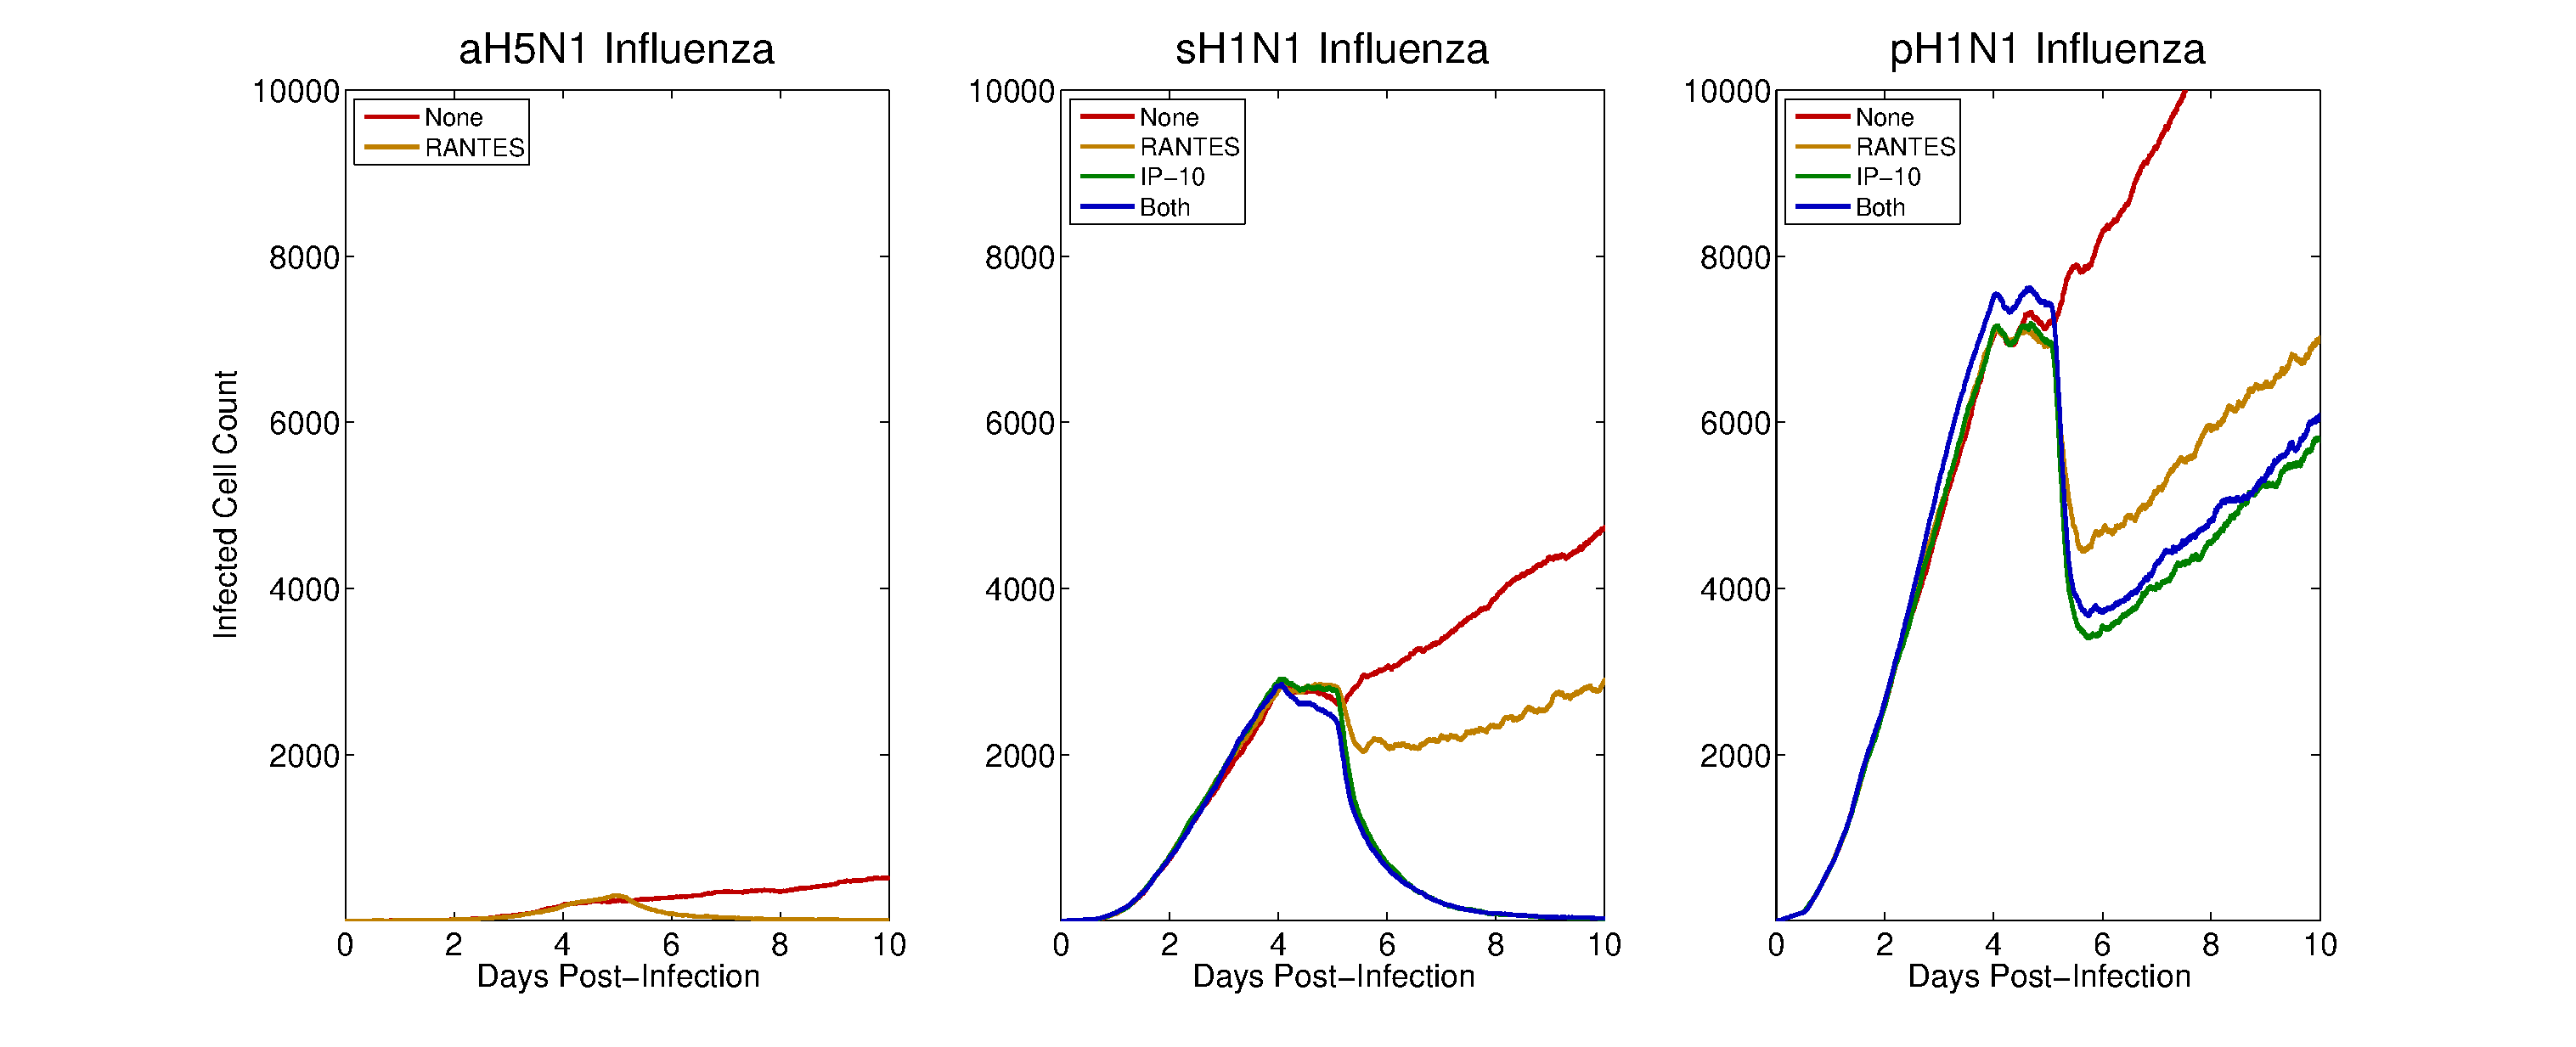
\includegraphics[width=\textwidth]{Figure_S2}
	\caption{\textbf{Effects of different chemokine combinations.}  A) aH5N1 does not stimulate an IP-10 response.  B-C) sH1N1 and pH1N1 show no significant difference between IP-10 alone versus IP-10 and RANTES combined.}
	\label{fig:chemokine}
\end{center}
\end{figure}

%\begin{figure}[ht!]
%\begin{center}
%	\includegraphics[width=\textwidth]{Figure_S3}
%	\caption{\drew{\textbf{Effects of different T cell speeds.}  With the exception of sH1N1, T cell speeds show a small effect during the early phase of the T cell response.  After a time of approximately two days, the infection dynamics converge to a similar rate of growth across all speed values.}}
%	\label{fig:speed}
%\end{center}
%\end{figure}

\setcounter{figure}{0}
\renewcommand{\figurename}{Video}


\begin{figure}[ht!]
\caption{The first of three overlaid videos of a representative seasonal H1N1 infection.  This video spans the 10 day infection and shows the cells as they transition from healthy to infected to dead.  T cells show half way through the simulation.  Healthy cells are gray, virus-incubating cells are yellow, virus-secreting cells are orange, apoptotic cells are red, and T cells are green.} 
 \label{video:cell_view}
\end{figure}

\begin{figure}[ht!]
\caption{The second of three overlaid videos of a representative seasonal H1N1 infection.  This video spans the 10 day infection and shows the virus concentration.  Notice the volatility when T cells arrive halfway through the simulation.  Virus concentration ranges from 1e-13 mols/mL (white) to 1e-27 mols/mL (black).  Refer to Figure 5 for the detailed legend. } 
 \label{video:virus_view}
\end{figure}

\begin{figure}[ht!]
\caption{The third of three overlaid videos of a representative seasonal H1N1 infection.  This video spans the 10 day infection and shows the chemokine concentration.  Notice the volatility when T cells arrive halfway through the simulation.  Chemokine concentration ranges from 1e8 ng/mL (white) to 1e-6 ng/mL (black).  Refer to Figure 5 for the detailed legend. } 
 \label{video:chemokine_view}
\end{figure}

\begin{figure}[ht!]
\caption{A closer look at the 2009 pandemic simulation.  This video shows the infection from day 6 to day 7 with each frame spanning 1 simulated minute.  Healthy cells are gray, virus-incubating cells are yellow, virus-secreting cells are orange, apoptotic cells are red, and T cells are green.  Note the high proportion of virus-secreting cells (orange) early on.  As time passes, secreting cells are gradually contained to the point where they become very sparse.  T cell clumping often prevents the T cells from quick discovery of new secreting cells.}
\end{figure}

\pagebreak

\section*{Tables}

%\begin{table}[!ht]
%\caption{
%\bf{Table title}}
%\begin{tabular}{|c|c|c|}
%table information
%\end{tabular}
%\begin{flushleft}Table caption
%\end{flushleft}
%\label{tab:label}

% \end{table}

\renewcommand{\thetable}{S\arabic{table}}

\begin{table}[!ht]
\begin{center}
\begin{tabular}{ | c | c | c | }
  \hline                        
  Paramter & Value & Source \\
  \hline
  T(0) & $1e6$ & \cite{Mitchell2011} \\
  V(0) &  $1e4$ & \cite{Mitchell2011} \\
  $r_{cell}$ &  $5 \mu m$ & \cite{Miao2010} \\
  $t_{rc}$ & $6s$ & \cite{Peters1983} \\
  $k_e$ & $6.4e-5/cell/day$ & \cite{Miao2010} \\
  $\beta$ & $4.8e-7/cell/PFU$ & \cite{Mitchell2011} \\
  $p$ & $0.18 PFU/h$ & \cite{Mitchell2011} \\
  $\delta$ & $16.7 hours$ & \cite{Mitchell2011} \\
  $a$ & $67.7$ & ABM fits \\
  $b$ & $433.5$ & ABM fits \\
  \hline  
\end{tabular}
\caption{Supplemental model parameters.  Most values are chosen to match the equations borrowed from both \cite{Mitchell2011} and \cite{Miao2010}.  Values \textit{a} and \textit{b} were fit to multiple runs of a simplified CyCells ABM.}
\label{table:supplement}
\end{center}
\end{table}

%\begin{table}[!ht]
%\begin{center}
%\begin{tabular}{ | c | c | }
%  \hline                        
%  Assumption & Description \\
%  \hline
%  2D hexagonal layout & The lung can be stretched flat.  T cells travel on the cellular surface. \\
%  Even blood flow to all capillaries & We assume that there is negligible increased blood flow to the infected region. \\
%  Rapid T cell circulation & Activated T cells in circulation do not spend time in new lymph nodes as they circulate. \\
%  T cell speed & T cells move at a rate of XXX in the absence of chemokine and XXXX once it detects chemokine. \\
%  T cell search time & T cells search in the lung for 6 minutes before they recirculate. \\
%  \hline  
%\end{tabular}
%\caption{Supplemental model parameters.  Most values are chosen to match the equations borrowed from both \cite{Mitchell2011} and \cite{Miao2010}.  Values \textit{a} and \textit{b} were fit to multiple runs of a simplified CyCells ABM.}
%\label{table:assumptions}
%\end{center}
%\end{table}

\end{document}
